% Energy based spectrum sensing
\section{Energy based Spectrum Detector for Multiple Primary Users}
\subsection{System Model}
We consider a cognitive radio system where the licensed frequency spectrum could be occupied by exactly one of two distinct OFDM signals $\{s_1, s_2\}$ or it could be vacant. Let $H_0$ denote the hypothesis under which the channel is free, ${H}_1$ denote the hypothesis under which the channel is occupied by $s_1$ and ${H}_2$ denote the hypothesis under which the channel is occupied by $s_2$. We are interested to test $H_0$ against $\bar{{H}_0}$.

A block diagram of the system is illustrate in Figure \ref{pic: block diagram}.

\begin{figure}[!hbp]
\centering
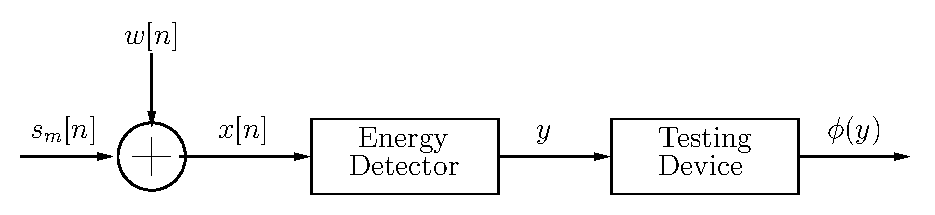
\includegraphics[width = \textwidth]{4/block_diagram.eps}
\caption{Block Diagram for Spectrum Sensing}
\label{pic: block diagram}
\end{figure}

The detector consists a measuring device followed by a testing device. 
The measuring device observes the noisy version of the signals that could present in the channel and outputs the sum energy of the sampled signals.
With this energy, the testing device employs MENP framework to decide the state of the channel.
The input to the measuring device is 
\begin{equation}
  x[n] = 
  \begin{cases}
	\omega[n]\;\;\;\;\;\;&\text{when ${H}_0$ is true}\\
	s_1[n]+\omega[n]\;\;\;\;\;\;&\text{when ${H}_1$ is true}\\
	s_2[n]+\omega[n]\;\;\;\;\;\;&\text{when ${H}_2$ is true}
  \end{cases}
\end{equation}
for $n = 0, \ldots, N-1$.
We assume  $s_i[n]\;\;(i=1, 2)$ and $\omega[n]$ are zero-mean independent and identically distributed (iid) circularly symmetric complex Gaussian (CSCG) random variables with variances $2\sigma_{s_i}^2\;\;(i=1, 2)$ and $2\sigma_{\omega}^2$, i.e., $s_m[n] \sim \mathcal{CN}(0, 2\sigma_{s_i}^2)\;\;(i=1, 2)$ and $\omega[n] \sim \mathcal{CN}(0, 2\sigma_{\omega}^2)$. 
Since the noise and signal are independent, $s_i[n]+\omega[n] \sim \mathcal{CN}(0, 2(\sigma_{s_i}^2 + \sigma_\omega^2))$.  Define $\sigma_0^2 = \sigma_\omega^2$ and $\sigma_i^2 = \sigma_{s_i}^2 + \sigma_\omega^2$, we can see
\begin{equation}
  \label{1129a1}
  \begin{split}
  \omega[n] &\sim \mathcal{CN}(0, 2\sigma_0^2)\\
  \omega[n] + s_1[n]&\sim \mathcal{CN}(0, 2\sigma_1^2)\\
  \omega[n] + s_2[n]&\sim \mathcal{CN}(0, 2\sigma_2^2) \,
  \end{split}
\end{equation}
for $n = 1, 2, \cdots, N-1$.  
The distribution of $x[n]$  can be written in form of
\begin{equation}
   \begin{split}
  H_0:\;\;\;\;\begin{pmatrix} x_R[n] \\ x_I[n] \end{pmatrix} \sim \mathcal{N}\Big( \begin{bmatrix} 0 \\ 0 \end{bmatrix}, \begin{bmatrix} \sigma_0^2 & 0\\ 0 & \sigma_0^2 \end{bmatrix} \Big)\\
  H_1:\;\;\;\;\begin{pmatrix} x_R[n] \\ x_I[n] \end{pmatrix} \sim \mathcal{N}\Big( \begin{bmatrix} 0 \\ 0 \end{bmatrix}, \begin{bmatrix} \sigma_1^2 & 0\\ 0 & \sigma_1^2 \end{bmatrix} \Big)\\
  H_2:\;\;\;\;\begin{pmatrix} x_R[n] \\ x_I[n] \end{pmatrix} \sim \mathcal{N}\Big( \begin{bmatrix} 0 \\ 0 \end{bmatrix}, \begin{bmatrix} \sigma_2^2 & 0\\ 0 & \sigma_2^2 \end{bmatrix} \Big)\,.  
\end{split}
  \label{equ:xdistribution}
\end{equation}
where $x_R[n]$ and $x_I[n]$ are real and imaginary part of signal $x[n]$.
Since the testing device outputs the energy of sampled signals, we have 
\begin{equation}
  y = \sum_{n=1}^{N}|x[n]|^2 = \sum_{n=1}^{N}(x_r[n]^2+x_i[n]^2)\,,
  \label{equ: testing device}
\end{equation}
Combine \eqref{equ:xdistribution} and \eqref{equ: testing device}, we can see 
\begin{equation} 
  \label{equ: abstract}
  \begin{split}
	H_0\;\;\;\;&\frac{y}{\sigma_0^2}\sim \mathcal{X}(2N)\\
	H_1\;\;\;\;&\frac{y}{\sigma_1^2}\sim \mathcal{X}(2N)\\
	H_2\;\;\;\;&\frac{y}{\sigma_2^2}\sim \mathcal{X}(2N)\,,
  \end{split}
\end{equation}
where $X(2N)$ is the Chi-square distribution with $2N$ degree freedom. 

Next we test $H_0$ against $\bar{H}_0$ using MENP framework. The problem can be abstract as
\begin{equation}
  \begin{split}
	\max\;\;\;\;&P_d\\
	\text{s.t.}\;\;\;\;&P_{f_1}\leq c_1\\
	&P_{f_2} \leq c_2\,.
  \end{split}
  \label{1129a3}
\end{equation}
Our goal is plot $P_d$ vs. $c_1, c_2$ (M-ROC) and find the decision rule for a given $c_1, c_2$ value.

From the definition of $\sigma_0^2, \sigma_1^2$ and $\sigma_2^2$, we know $\sigma_0^2 < \sigma_1^2, \sigma_2^2$. Hence  problem given in \eqref{1129a3} has the same form as that of Chi-Square Example given in last chapter. From the conclusion in last chapter, the optimal  decision rule for a given $c_1, c_2$ is 
\begin{equation}
  x \substack{H_0 \\ < \\ > \\ \bar{H}_0} x_0
  \label{equ:1129a4}
\end{equation}
where $x_0 = \min\{F_1^{-1}(c_1),  F_2^{-1}(c_2)\}$ and $F_1. F_2$ are the CDFs of $y$ under hypothesis $H_1, H_2$ respectively. The expression of $P_d$ is 
\begin{equation}
  P_d = F_0(x_0)\,.
  \label{equ:1129a5}
\end{equation}

We use Matlab to compute the M-ROC for this energy detector. The value of $c_1, c_2$ range from 0 to 1 with step 0.01. By using \eqref{equ:1129a4} and \eqref{equ:1129a5}, the value of $P_d$ can be acquired. The M-ROC is illustrate in 
